\section{Análise Estatística de Dados}
\label{sec:ref-analise-dados}

Esta seção aborda os conceitos e metodologias do domínio da estatística necessários para testes de hipótese. O propósito é realizar uma contextualização nas metodologias que serão empregadas durante a análise dos dados quantitativos durante o estudo de caso deste trabalho.

Para a realização de decisões estatísticas, são formuladas \textbf{hipóteses estatísticas}, que servem para guiar a avaliação de amostras de dados coletadas, bem como tomadas de decisão. Em um experimento, estas hipóteses são definidas na fase de planejamento e devem guiar todo o processo de experimentação. Quando desejamos analisar a diferença entre duas amostras, formulamos hipóteses para que as mesmas sejam aceitas ou rejeitadas, iniciando pela proposição de que não há diferença entre as amostras. Esta hipótese inicial é chamada de \textbf{hipótese nula}, já as demais são chamadas \textbf{hipóteses alternativas} \cite{juristo_basics_2001}.

Visando rejeitar a hipótese nula, se analisa a diferença entre as amostras coletadas e, caso esta seja considerável, entende-se que é \textit{significativa} e suficiente para a tomada de decisão. As maneiras pelas quais medimos este nível de diferença são chamadas de \textbf{testes de significância} ou \textbf{regras de decisão} \cite{juristo_basics_2001}.

Quando a hipótese nula é rejeitada quando não deveria, se caracteriza um \textbf{erro do tipo I}, ou seja, um falso positivo. Quando o contrário acontece e a hipótese nula é aceita quando não deveria, um falso negativo, se tem um \textbf{erro do tipo II}. O risco de acontecimento de ambos os erros podem ser mitigados através do aumento da amostra, porém, isso nem sempre é possivel \cite{wohlin_experimentation_2012}.

Ao se realizar um teste de hipótese, é definido um \textbf{nível de significância}, que seria o nível máximo que o pesquisador está disposto a arriscar cometer um erro de tipo I. Ou seja, caso seja definido um nível de 0.05 (5\%), é aceito que a cada 100 análises, 5 rejeitarão a hipótese nula quando ela deveria ser aceita. Normalmente este nível é representado pela letra grega alfa (\( \alpha \)) \cite{juristo_basics_2001}.

Já os erros de tipo II dependem de outros fatores, como a diferença nas observações das diferentes hipóteses e poder do teste estatístico, representada por beta (\( \beta \)). O \textbf{poder de um teste} é definido pela probabilidade de se rejeitar corretamente a hipótese nula, representado por 1 - \( \beta \). Por exemplo, um nível de poder de 0.4 indica que se um experimento for executado 10 vezes um efeito causado por algum fator alternativo será descoberto apenas em 4 delas \cite{juristo_basics_2001}.

\subsection{Estatística Descritiva}
\label{subsec:descritiva}

Após a coleta dos dados, pode se utilizar de métodos de estatística descritiva para se apresentar e descrever estes conjuntos, visando entender sua natureza e identificar anomalias. O objetivo é observar a distribuição do conjunto, se há dados que podem ser desconsiderados e decidir o teste de hipótese mais adequado para a comparação das amostras \cite{wohlin_experimentation_2012}.

\subsubsection{Medidas de Tendência Central e de Distribuição}

\citeonline{wohlin_experimentation_2012} definem que as medidas de tendência central visam apontar o centro do conjunto de dados, e que para isso utilizam os valores de \textbf{média (\( \overline{x} \))}, que é soma dos valores divida pela sua quantidade, \textbf{moda}, que se trata do valor mais recorrente do conjunto e \textbf{mediana (\( \tilde{x} \))}, que seria o valor encontrado no meio do conjunto após sua ordenação.

A mediana, também pode ser representada como \(x_{50\%}\), o que indica que ela é o percentil 50\%. Um \textbf{percentil} \(x_p\) indica o valor abaixo do qual \(p\%\) dos dados se encontram. Existem casos especiais de percentis chamados \textbf{quartis}, que dividem os dados em quatro partes iguais: o primeiro quartil (Q1 ou \(l_q\)) marca o valor abaixo do qual se encontra 25\% dos dados amostrais, e o terceiro quartil (Q3 ou \(u_q\)), 75\% \cite{wohlin_experimentation_2012}.

\citeonline{wohlin_experimentation_2012} também apresentam as medidas de distribuição, que por sua vez visam apresentar quão concentrado está o conjunto de dados. Para isto utiliza-se de medidas como a \textbf{variância (\textit{\( s^2 \)})}, o \textbf{desvio padrão (\textit{s})} e a \textbf{amplitude}. A amplitude é a distância entre os valores máximos e mínimos do conjunto. A variância é a média dos quadrados das distâncias entre os valores da amostra e sua média. O desvio padrão é a raiz quadrada da variância. Então, sendo \textit{s} o desvio padrão, \( s^2 \) a variância, \textit{n} o número de dados observados e \(x_i \) o i-ésimo dado observado, as medidas citadas podem ser representadas da seguinte forma:
\[
\text{amplitude} = x_{\text{max}} - x_{\text{min}}
\]

\[
\textit{s} = \sqrt{s^2}
\]

\[
s^2 = \frac{1}{n} \sum_{i=1}^{n} (x_i - \bar{x})^2
\]


\subsubsection{Representação Gráfica}

Além das medidas existentes na estatística descritiva, \citeonline{wohlin_experimentation_2012} também abordam como a representação gráfica do conjunto de dados pode ajudar a entender a natureza do conjunto, ajudando a identificar visualmente \textit{outliers}, que são pontos que diferem muito do conjunto e atrapalhar a análise. Os autores apresentam diferentes tipos de gráficos que podem ser úteis para esta prática, alguns deles são:

\begin{itemize}
    \item \textbf{Gráfico de Dispersão:} apresenta amostras pareadas em duas dimensões, permitindo identificar dependências, padrões lineares e \textit{outliers} (exemplificado na Figura \ref{fig:scatterplot});
    \item \textbf{Gráfico de Caixa (\textit{Box Plot}):} permite se visualizar a dispersão e a assimetria dos dados. Apresenta a mediana, o primeiro e o terceiro quartis (exemplificado na Figura \ref{fig:boxplot}). A largura da caixa é \textit{d} onde \textit{d} = \(u_q\) - \(l_q\). O gráfico é delimitado por suas caudas (ou bigodes), que se estendem até 1,5 vezes o comprimento da caixa a partir dos quartis. Esta delimitação serve para representar a área onde, teoricamente, todos os dados conjunto deveriam ser encontrados, ou seja, aqueles fora desta região são considerados \textit{outliers}; e
    \item \textbf{Histograma:} representa a distribuição dos dados e mostra a frequência de intervalos de valores (exemplificado na Figura \ref{fig:histogram}). Cada barra representa a quantidade de dados dentro de um intervalo específico e sua altura indica a frequência de dados dentro deste intervalo. Isto permite observar facilmente a distribuição que os dados seguem ou se existem picos ou lacunas significativas.
\end{itemize}

\begin{figure}
    \centering
    
    \caption{Exemplo de Gráfico de Dispersão}
    
    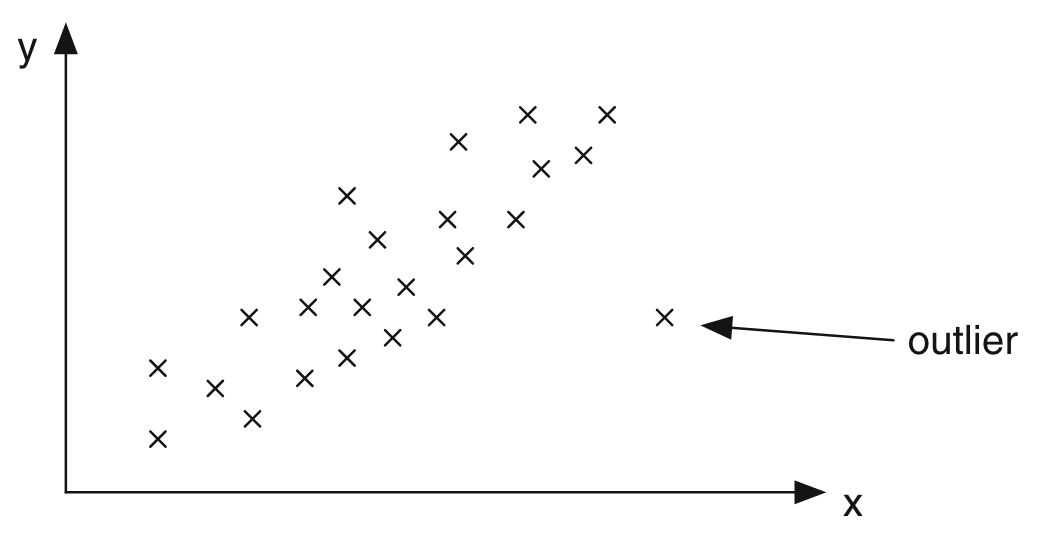
\includegraphics[width=0.7\linewidth]{figuras/scatter.png}
    
    \text{Fonte: \citeonline{wohlin_experimentation_2012}}
    
    \label{fig:scatterplot}
\end{figure}

\begin{figure}
    \centering
    
    \caption{Exemplo de Gráfico de Caixa}
    
    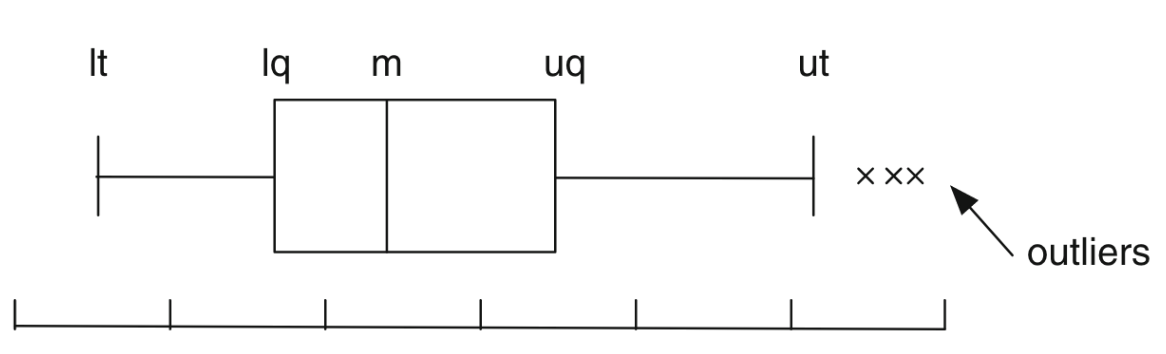
\includegraphics[width=0.7\linewidth]{figuras/boxplot.png}
    
    \text{Fonte: \citeonline{wohlin_experimentation_2012}}
    
    \label{fig:boxplot}
\end{figure}

\begin{figure}
    \centering
    
    \caption{Exemplo de Histograma}
    
    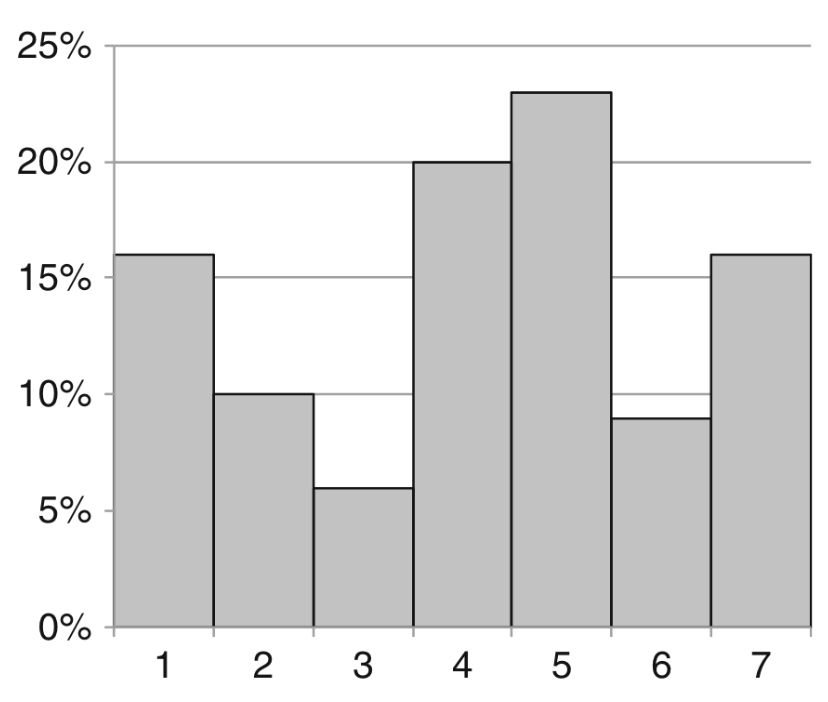
\includegraphics[width=0.5\linewidth]{figuras/histogram.png}
    
    \text{Fonte: \citeonline{wohlin_experimentation_2012}}
    
    \label{fig:histogram}
\end{figure}

A identificação dos \textit{outliers} por meio destes processos de representação gráfica é crucial para a chamada \textbf{redução dos dados}. Valores que se desviam significativamente dos demais podem comprometer a qualidade do conjunto de dados e prejudicar a análise. Portanto, é fundamental identificá-los e avaliar a necessidade de sua remoção. Caso um valor resulte de um evento raro, ele pode ser removido; no entanto, um ponto que revele informações valiosas deve ser analisado separadamente \cite{wohlin_experimentation_2012}.

\subsection{Teste de Hipóteses}

O objetivo de um teste de hipótese é verificar se é possível rejeitar uma hipótese nula a partir da análise de um determinado conjunto de dados. Ou seja, \(x_i \) descreve determinadas propriedades e o teste visa negar estas características com determinado nível de significância \cite{wohlin_experimentation_2012}. 

Um teste de hipótese pode ser paramétrico ou não paramétrico. Os paramétricos se baseiam em modelos que pressupõem a distribuição dos dados coletados, já os não paramétricos não fazem suposições \cite{juristo_basics_2001}. Um destes pressupostos pode ser que o conjunto está normalmente distribuído. Esta distribuição é caracterizada por uma curva simétrica em formato de sino e isso pode ser verificado através de diferentes tipos de gráficos \cite{wohlin_experimentation_2012}.

A seguir serão apresentados alguns testes de hipótese existentes, métodos que se adequam ao contexto deste trabalho, onde serão avaliadas amostras independentes de dados, que podem ser grandes ou pequenas e que podem ter sua distribuição normal ou não.

\subsubsection{Teste Z}

Este é um teste paramétrico para quando trabalhamos com amostras grandes (\(n \geq 30\)). Nestes conjuntos a distribuição das médias amostrais tende a ser normal, o que significa que a média das amostras se aproxima da média da população total, assim como o desvio padrão. Isso facilita a inferência sobre a população total com base nos dados coletados \cite{juristo_basics_2001}.

Utiliza-se da regra de decisão de diferença entre médias para se avaliar a significância da diferença entre as duas amostras coletadas. Caso essa diferença não seja significativa, se entende que a diferença observada pode ser atribuída ao acaso, o que nos leva a não rejeitar a hipótese nula. O valor responsável por nos dizer o valor dessa significância é chamada de z (ou \textit{z-score}) \cite{juristo_basics_2001}.

\citeonline{juristo_basics_2001} demonstram que para calcular o valor de \textit{z}, primeiro realizamos um processo de normalização dos valores da amostra analisada, para que possamos distribuir nossos dados na distribuição padrão da variável \textit{z}, apresentada na Figura \ref{fig:z-score} (onde a média é 0 e o desvio padrão é 1). Nesta curva, o valor central é 0, e o eixo x tem como medida o desvio padrão, que no caso é 1, o valor de \textit{z} vai nos dizer quantos desvios padrões um dado valor se distancia da média, que é 0. 

Para calcular o valor de \textit{z} se utiliza a seguinte fórmula, onde \textit{S} é alguma medida da amostra (média, desvio padrão, etc), e \(\mu_S\) e \(\sigma_S\) são respectivamente a média e o desvio padrão desta medida:

\[
z = \frac{S - \mu_S}{\sigma_S}
\]

Assim, os valores mais distantes se encontram nas regiões críticas, como apresentado na Figure \ref{fig:z-score}, que demonstra que os valores encontrados nelas teriam um \textit{z-score} maior que 1.96 ou menor que -1.96 (no exemplo o nível de significância é de 0.05, ou 5\%).



\begin{figure}
    \centering
    
    \caption{Distribuição da Estatística Z}
    
    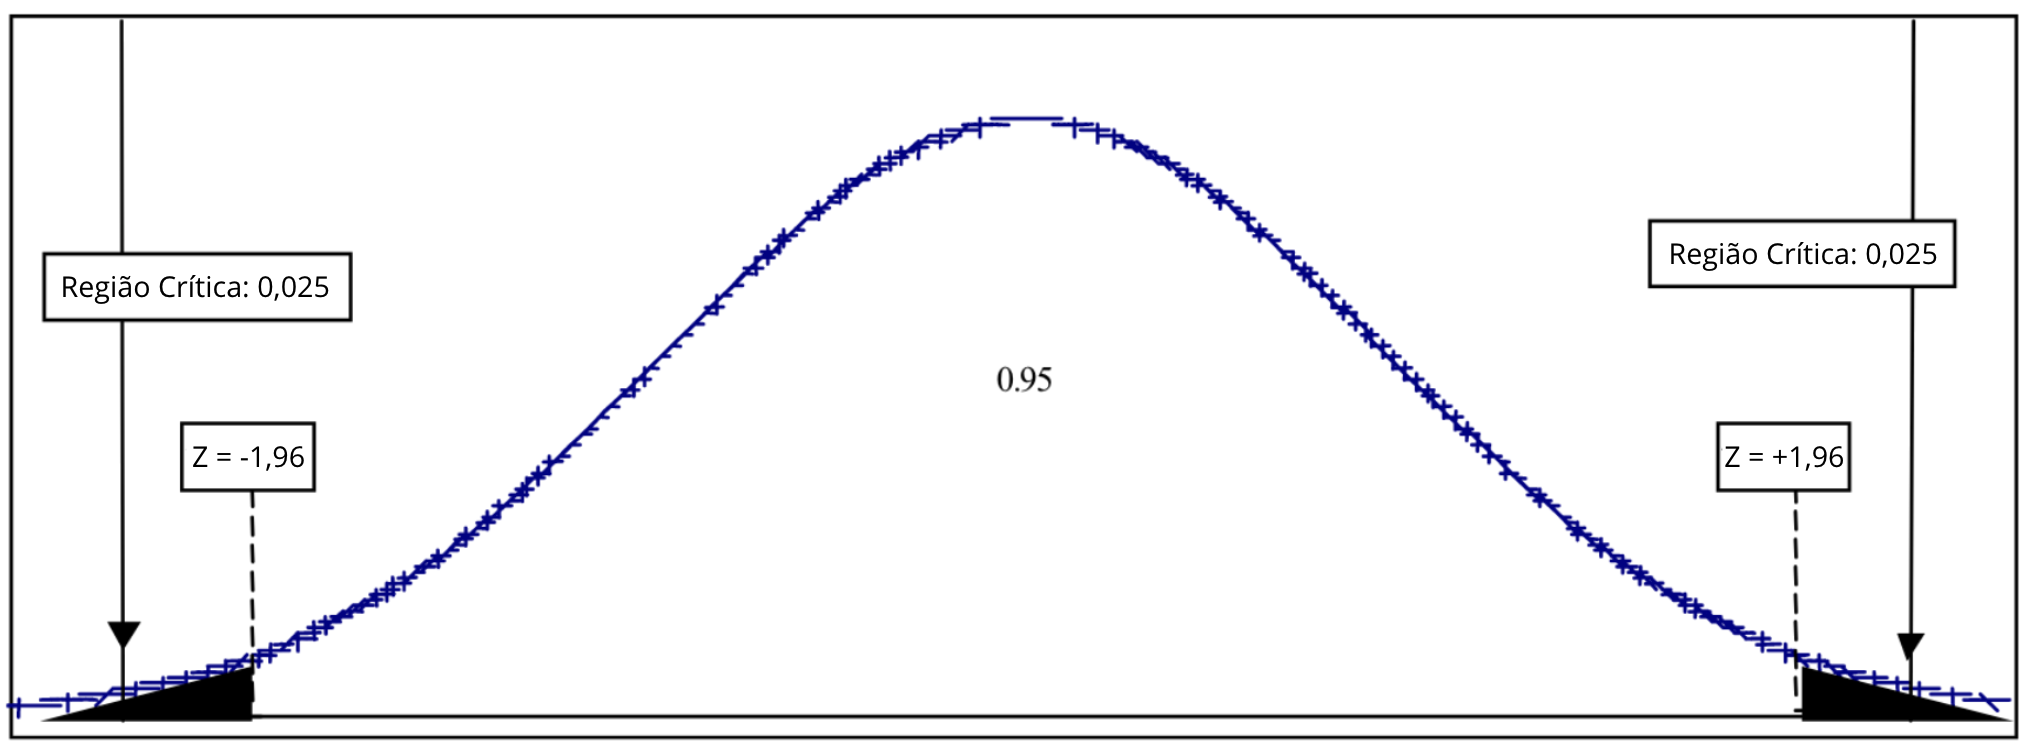
\includegraphics[width=1\linewidth]{figuras/z_distr.png}
    
    \text{Fonte: Adaptado de \citeonline{juristo_basics_2001}}
    
    \label{fig:z-score}
\end{figure}

\subsubsection{Teste T de Student}
\label{subsec:t-test}

Este também é um teste paramétrico, onde se espera que a amostra coletada se aproxime da distribuição normal. É uma alternativa para quando se lida com conjuntos pequenos de dados. A distribuição do valor de \textit{t} é bem parecida com a distribuição normal, porém depende do grau de liberdade da amostra, que é representado por \textit{v}. Quanto maior o grau de liberdade, mais a curva da distribuição se aproxima da curva normal \cite{juristo_basics_2001}. Esse teste é comumente utilizado para comparar duas amostras independentes de variáveis numéricas \cite{wohlin_experimentation_2012}.

A curtose é uma característica da estatística descritiva que define o achatamento da curva de uma distribuição. A curtose de uma distribuição normal é 0, indicando uma distribuição com um formato de sino padrão. Em contraste, a curtose de uma distribuição t de Student tende a ser cada vez mais negativa conforme o grau de liberdade diminui \cite{juristo_basics_2001}. Isso significa que, com menos graus de liberdade, a distribuição t apresenta caudas mais largas e uma forma mais achatada, refletindo a maior variabilidade e incerteza associadas a amostras menores, vide a Figura\ref{fig:t-statistic}.

O grau de liberdade é calculado a partir da quantidade de amostras a serem testadas e seus respectivos tamanhos, sendo uma amostra \textit{v} = \textit{n} - 1, para duas amostras \textit{v} = \textit{\(n_1\)} + \textit{\(n_2\)} - 2 e assim sucessivamente \cite{juristo_basics_2001}.



\begin{figure}
    \centering
    
    \caption{Distribuição de T Para Diferentes Graus de Liberdade}
    
    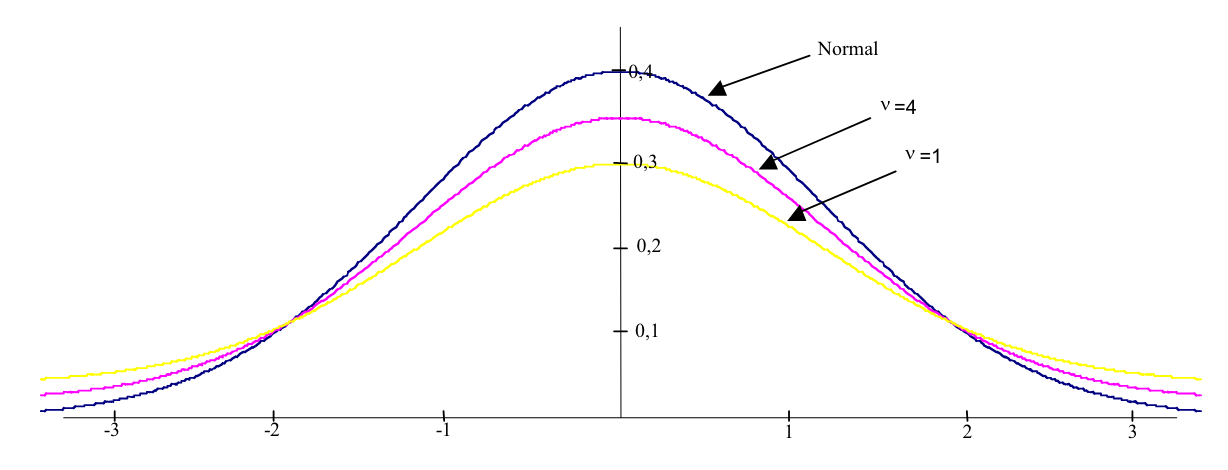
\includegraphics[width=1\linewidth]{figuras/t-statistic.png}
    
    \text{Fonte: \citeonline{juristo_basics_2001}}
    
    \label{fig:t-statistic}
\end{figure}


Para se calcular o valor \textit{t} utiliza-se a fórmula:

\[
t = \frac{\bar{x} - \mu}{s / \sqrt{n}}
\]

onde \(\bar{x}\) é a média amostral, \(\mu\) é a média da população (ou a média de outra amostra), \(s\) é o desvio padrão amostral e \(n\) é o tamanho da amostra. O valor calculado de t é então comparado com os valores críticos da tabela t, que são ajustados para diferentes níveis de significância e graus de liberdade. Esses valores críticos ajudam a determinar se a diferença observada é estatisticamente significativa. A tabela t de Student é gerada a partir de cálculos que levam em consideração a distribuição das amostras \cite{juristo_basics_2001}.




\subsubsection{Teste de Mann-Whitney U}
\label{subsec:u-test}

O teste de Mann-Whitney U, também conhecido como teste U, é uma alternativa não paramétrica para a análise de duas amostras. Este teste não assume que os dados seguem uma distribuição normal, tornando-o mais flexível e aplicável a dados medidos em escalas ordinais. O teste é utilizado para determinar se há uma diferença significativa entre duas amostras independentes \cite{wohlin_experimentation_2012}.

\citeonline{juristo_basics_2001} demonstram que para se realizar o teste de Mann-Whitney U, as observações das duas amostras são organizadas em ordem crescente e substituídas pelos seus postos ou \textit{ranks}. Quando há empates, cada valor é substituído pela média dos \textit{ranks} correspondentes. A soma dos \textit{ranks} para cada amostra é calculada e utilizada para determinar o valor da estatística \textit{u}. A fórmula para o cálculo de \textit{u} é:

\[
u = r_1 - \frac{n_1 (n_1 + 1)}{2}
\]

onde \(r_1\) é a soma dos \textit{ranks} da primeira amostra e \(n_1\) é o número de observações na primeira amostra. A distribuição amostral de \(u\) é simétrica e, quando o tamanho das amostras é suficientemente grande (geralmente \(n_1 \geq 8\) e \(n_2 \geq 8\)), a distribuição de \(u\) pode ser aproximada por uma distribuição normal com média (\(\bar{x}\)) e variância (\textit{s}) dadas por:

\[
\bar{x} = \frac{N_1 N_2}{2}
\]
\[
\text{s} = \frac{n_1 n_2 (n_1 + n_2 + 1)}{12}
\]

O valor \(z\) é calculado como:

\[
z = \frac{u - \bar{x}}{s}
\]

Esse valor \(z\) é então comparado com os valores críticos da tabela padrão normal para determinar se a diferença observada entre as amostras é estatisticamente significativa. Se \(z\) cair fora do intervalo crítico definido (por exemplo, -1.96 a 1.96 para um nível de significância de 0.05), rejeita-se a hipótese nula e conclui-se que há uma diferença significativa entre as amostras \cite{juristo_basics_2001}.

\subsubsection{Teste Qui-Quadrado}
\label{subsec:chi-square}

O teste qui-quadrado também é um teste não paramétrico. É utilizado para analisar a diferença entre as frequências observadas e esperadas de uma variável categórica. O objetivo do teste é verificar se há uma diferença significativa entre as frequências esperadas, sob uma hipótese nula \(h_0\), e as frequências observadas. É um teste indicado para amostras grandes, diferindo do Mann-Whitney, que é mais apropriado para amostras pequenas \cite{juristo_basics_2001}. Para realização deste teste se utiliza a estatística qui-quadrado (\(\chi^2\)), que é calculada usando a seguinte fórmula:

\[
\chi^2 = \sum_{i=1}^{k} \frac{(o_i - e_i)^2}{e_i}
\]

onde \(o_i\) são as frequências observadas, \(e_i\) são as frequências esperadas sob a hipótese nula, e \(k\) é o número de eventos ou categorias. O valor calculado de \(\chi^2\) é então comparado a um valor crítico da tabela qui-quadrado, que varia de acordo com o número de graus de liberdade (\(\nu = k - 1\)) e o nível de significância escolhido \cite{juristo_basics_2001}.

Se o valor calculado de \(\chi^2\) for maior que o valor crítico da tabela (como \(\chi^2_{0.95}\), para um nível de significância de 0,05), a hipótese nula é rejeitada, indicando uma diferença significativa entre as frequências observadas e esperadas. Caso contrário, não há evidência suficiente para rejeitar a hipótese nula \cite{juristo_basics_2001}.
